\documentclass[a4paper,12pt]{article}
\usepackage{graphicx}
\usepackage{hyperref}
\usepackage{amsmath}
\usepackage{amssymb}
\usepackage{geometry}
\usepackage{cite}
\usepackage{tikz}
\usepackage{braket}
\usepackage{tikz-3dplot}

\geometry{margin=1in}

\title{\textbf{Quantum Computing: The Future of Computation}}
\author{\textbf{Student Name:} Your Name \\ 
    \textbf{Roll Number:} Your Roll No \\ 
    \textbf{Guide:} Faculty Name \\ 
    \textbf{Department of Computer Science and Engineering}}
\date{\today}

\begin{document}

\maketitle

\section{Seminar Topic}
\textbf{Quantum Computing: Principles and Applications}

\section{Index / Contents of Presentation}
\begin{enumerate}
    \item Seminar Topic
    \item Student Details
    \item Index / Contents of Presentation
    \item Abstract / Aim
    \item Introduction
    \item Background / Existing Systems
    \item Drawbacks of Classical Computing
    \item Quantum Computing: Concepts \& Principles
    \item Quantum Bits (Qubits) and Superposition
    \item Quantum Entanglement and Quantum Gates
    \item Quantum Algorithms (Shor’s Algorithm, Grover’s Algorithm)
    \item Quantum Hardware \& Real-World Implementations
    \item Advantages \& Applications
    \item Future Enhancements \& Challenges
    \item Conclusion
    \item References
\end{enumerate}

\section{Abstract / Aim}
Quantum computing is a revolutionary technology that leverages quantum mechanics principles such as superposition and entanglement to perform computations exponentially faster than classical computers. This seminar explores the fundamentals, applications, and future implications of quantum computing in fields like cryptography, AI, and optimization problems.

\section{Introduction}
Traditional computers rely on binary bits (0s and 1s) to process data. Quantum computers use qubits, which can exist in multiple states simultaneously due to superposition. This enables quantum computers to solve complex problems much faster than classical computers.

\section{Background / Existing Systems}
Classical computers use transistors and logic gates for data processing. However, they face limitations in processing power and exponential complexity. Moore’s Law is slowing down, and quantum computing presents an alternative approach to computational problems.

\section{Drawbacks of Classical Computing}
\begin{itemize}
    \item Inefficiency in solving complex problems (e.g., cryptography, simulations).
    \item High energy consumption for large-scale computing tasks.
    \item Scaling limits due to transistor miniaturization.
\end{itemize}

\section{Quantum Computing: Concepts \& Principles}
Quantum computing is based on:
\begin{itemize}
    \item \textbf{Superposition}: A qubit can be both 0 and 1 simultaneously.
    \item \textbf{Entanglement}: Two qubits can be linked, allowing instant information exchange.
    \item \textbf{Quantum Gates}: Unlike classical AND/OR gates, quantum gates like Hadamard, CNOT, and Toffoli are used.
\end{itemize}

\section{Quantum Bits (Qubits) and Superposition}
Qubits, the fundamental units of quantum computation, can exist in a combination of states, allowing parallel computation and faster problem-solving.

Traditional computers rely on binary bits (0s and 1s) to process data. Quantum computers use qubits, which can exist in multiple states simultaneously due to superposition. This enables quantum computers to solve complex problems much faster than classical computers \cite{Gruska}.

\begin{figure}[ht]
    \centering
    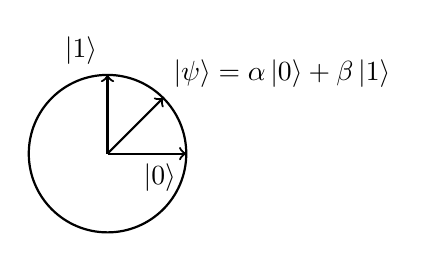
\begin{tikzpicture}
    \draw[thick] (0,0) circle (1);
    \draw[thick,->] (0,0) -- (0.707,0.707) node[anchor=south west] {$\ket{\psi} = \alpha\ket{0} + \beta\ket{1}$};
    \draw[thick,->] (0,0) -- (1,0) node[anchor=north east] {$\ket{0}$};
    \draw[thick,->] (0,0) -- (0,1) node[anchor=south east] {$\ket{1}$};
    \end{tikzpicture}
    \caption{Qubit representation on the Bloch sphere. Reprinted from Programming for the quantum computer (Dickel, 2016)}
    \label{fig:qubit}
\end{figure}

\begin{figure}[ht]
    \centering
    \tdplotsetmaincoords{60}{120}
    \begin{tikzpicture}[tdplot_main_coords]
        \draw[thick,->] (0,0,0) -- (3,0,0) node[anchor=north east]{$x$};
        \draw[thick,->] (0,0,0) -- (0,3,0) node[anchor=north west]{$y$};
        \draw[thick,->] (0,0,0) -- (0,0,3) node[anchor=south]{$z$};
        \draw[thick,->] (0,0,0) -- (1,1,1) node[anchor=south]{$\ket{\psi}$};
        \draw[dashed] (1,1,1) -- (1,1,0);
        \draw[dashed] (1,1,1) -- (1,0,1);
        \draw[dashed] (1,1,1) -- (0,1,1);
    \end{tikzpicture}
    \caption{3D representation of a qubit state. Reprinted from Programming for the quantum computer (Dickel, 2016)}
    \label{fig:qubit3d}
\end{figure}

\section{Quantum Entanglement and Quantum Gates}
Entanglement is a phenomenon where qubits are interdependent. Quantum gates manipulate qubits, enabling quantum algorithms to process data efficiently \cite{Gruska}.

\section{Quantum Gates}
Quantum gates are the building blocks of quantum circuits, similar to logic gates in classical computing. They operate on qubits to perform quantum operations.

\subsection{Hadamard Gate (H)}
The Hadamard gate creates superposition by transforming a qubit's state:
\begin{equation}
H = \frac{1}{\sqrt{2}}
\begin{bmatrix} 1 & 1 \\ 1 & -1 \end{bmatrix}
\end{equation}
It converts $|0\rangle$ into $(|0\rangle + |1\rangle)/\sqrt{2}$ and $|1\rangle$ into $(|0\rangle - |1\rangle)/\sqrt{2}$.

\subsection{Pauli Gates (X, Y, Z)}
These gates represent quantum analogs of classical NOT and phase flip operations.
\begin{itemize}
    \item \textbf{Pauli-X (NOT Gate)}:
    \begin{equation} X = \begin{bmatrix} 0 & 1 \\ 1 & 0 \end{bmatrix} \end{equation}
    Swaps $|0\rangle$ and $|1\rangle$.
    \item \textbf{Pauli-Y}:
    \begin{equation} Y = \begin{bmatrix} 0 & -i \\ i & 0 \end{bmatrix} \end{equation}
    Adds a phase shift and swaps qubits.
    \item \textbf{Pauli-Z (Phase Flip)}:
    \begin{equation} Z = \begin{bmatrix} 1 & 0 \\ 0 & -1 \end{bmatrix} \end{equation}
    Introduces a phase shift to $|1\rangle$.
\end{itemize}

\subsection{CNOT (Controlled-NOT) Gate}
The CNOT gate flips the target qubit if the control qubit is $|1\rangle$:
\begin{equation}
CNOT = \begin{bmatrix} 1 & 0 & 0 & 0 \\ 0 & 1 & 0 & 0 \\ 0 & 0 & 0 & 1 \\ 0 & 0 & 1 & 0 \end{bmatrix}
\end{equation}
Used in entanglement generation.

\subsection{Toffoli (CCNOT) Gate}
A three-qubit gate that flips the third qubit if the first two are $|1\rangle$.

\subsection{SWAP Gate}
Interchanges two qubits:
\begin{equation}
SWAP = \begin{bmatrix} 1 & 0 & 0 & 0 \\ 0 & 0 & 1 & 0 \\ 0 & 1 & 0 & 0 \\ 0 & 0 & 0 & 1 \end{bmatrix}
\end{equation}

\subsection{Fredkin (CSWAP) Gate}
A three-qubit gate that swaps two qubits only if the control qubit is $|1\rangle$.

\subsection{Phase Shift Gates}
These introduce a phase factor:
\begin{equation} P(\theta) = \begin{bmatrix} 1 & 0 \\ 0 & e^{i\theta} \end{bmatrix} \end{equation}
Examples include the $S$ and $T$ gates, where $S=P(\pi/2)$ and $T=P(\pi/4)$.

\section{Quantum Algorithms}
\subsection{Shor’s Algorithm}
Shor’s algorithm efficiently factors large numbers, posing a threat to current encryption systems.

\subsection{Grover’s Algorithm}
Grover’s algorithm speeds up search problems significantly by reducing time complexity.

\section{Quantum Hardware \& Real-World Implementations}
Companies like IBM, Google, and D-Wave are developing quantum processors, with IBM Quantum Experience offering cloud-based quantum computing.

\section{Advantages \& Applications}
\begin{itemize}
    \item Cryptography and Cybersecurity
    \item Artificial Intelligence and Machine Learning
    \item Drug Discovery and Material Science
    \item Financial Modeling and Risk Analysis
    \item Weather Prediction and Climate Modeling
\end{itemize}

\section{Future Enhancements \& Challenges}
\begin{itemize}
    \item Scalability Issues: Difficulty in building large quantum computers.
    \item Error Correction: Qubits are fragile and require quantum error correction.
    \item High Cost: Quantum hardware requires ultra-cold environments.
    \item Algorithm Development: Need for more quantum algorithms for real-world applications.
\end{itemize}

\section{Conclusion}
Quantum computing has the potential to revolutionize technology. Advancements in quantum hardware and algorithms will shape the future of computation. While challenges remain, continuous research promises significant breakthroughs.

\section{References}
\begin{itemize}
    \item M. A. Nielsen, I. L. Chuang, \textit{Quantum Computation and Quantum Information}.
    \item Research papers from IBM Quantum Experience.
    \item MIT OpenCourseWare lectures on Quantum Computing.
    \item J. Gruska, \textit{Quantum Computing}.
\end{itemize}

\end{document}
